\section{區議員的職責不就是服務街坊,為何要政治化?}

區議員的職責不止於街坊服務,還有很多政治功能。而公眾以為區議員的職責只不過是服務街坊,忽略他們的政治功能,本身就是一個高度政治化操作的結果,後面涉及龐大的政治和金錢利益。

香港目前有兩級議會,即立法會和區議會。立法會議員的政治公作,例如監察政府施政和辯論公共議題,公眾很多時候都能在主流傳媒看得到。不過立法會議員只有七十名,區議員卻有四百多名,而且分開十八個區議會開會,主流傳媒便少有機會報道他們的議會工作。與此同時,因為區議會的選區比較細少,公眾日常生活接觸區議員的機會比較多,於是乎便很容易誤以為區議員的工作限於服務當區居民,例如舉辦敬老活動或巡視街道衛生等。

現實上,區議員有很多直接和全港政治相關的工作。首先,選舉行政長官的1200名選舉委員會成員當中,有117人由區議員互選產生,佔整體接近十分之一,人數也是選舉委員會各組成界別當中最多。由於這些委員是互選產生,也就是說只要某政治陣營能夠連結全港半數的區議員,就可以一次過在選舉委員會拿走117票。這種對行政長官舉足輕重的影響力,在區議會選舉很少會被提及,也很少選民在區議會投票時會想到他們正在間接參與行政長官選舉。

此外,政府近年經常利用「區議會包圍立法會」的策略,把一些和當區不相關的全港性議題交給各個區議會討論,然後以「得到十八區區議會支持」來說明政府已得到民意支持。近年以此策略在區議會層面動員支持的做法,包括支持廣深港高速鐵路於西九龍站實施「一地兩檢」和支持人大常委就行政長官普選辦法的決定(即「八三一決定」)。此外,每當政府要為一些全港性政策做大型諮詢,也會到各區區議會聽取意見,例如優化土地供應策略或自願醫保計劃等等。和行政長官選舉一樣,區議會選舉的候選人在這些全港性議題的立場很少會被關注,但他們當選後卻可代表市民在這些題目上協助政府製造民意支持。

直接點說,區議員有很明確的政治功能,而當選民投票選區議員的時候忽視這些政治功能,就等於為他們日後如何運用其政治影響力開了一張沒有銀碼的支票,讓他們隨意利用自己的政治角色。

為什麼公眾會以為區議員的工作不涉政治?這點既和選舉制度有關,也有政治力量的刻意安排。香港分十八個區議會,每區再分十多到三十多個小選區,每區人口約一萬多,以簡單多數制選出一名區議員。每次選舉中會去投票的,一般是三千到六千人左右。簡單多數制會鼓勵每區只得兩名候選人競爭,以免出現漁人得利的情況。因此,區議會選舉的勝負往往只有數百票之差,於是選戰很容易會變成人際關係的比併。由於香港人口稠密,每個選區可能只有四、五個街區或一條公共屋邨的規模,加上前面提到主流傳媒很少會報道個別區議員的工作,選民是否直接看得見候選人本身就變得很重要,為選民提供個人服務就成為了競選工程的必然起點。

所謂選民服務,很多時候是指為老人量血壓、幫學生拍證件照,又或搞街坊旅行團等活動,後面的目的都是要搜集選民的聯絡方式,以便建立關係和日後拉票。因為成年人往往要外出工作,加上香港工時長而且往往上班路途遙遠,所以留在社區中的時間未必很多。相反,退休老人在社區中的時間明顯較多,成為區議員拉關係的重點對象。不少區議員都會針對老年人的需要,按時節派發各種禮物,例如端午節派糭或者中秋節派月餅,統稱「蛇齋餅糭」(蛇宴、齋宴、月餅、糭)來建立支持者網絡。而區議會的活動經費,則往往會用來辦一些內容沒有多大分別的「交通安全嘉年華」或「滅罪嘉年華」,結果都是找個理由搭起舞台然後弄些表演節目給老年人看,有前區議員稱之為「舞台社區」。

接下來,就是一連串劣幣驅逐良幣的過程。想花心思做社區充權的往往會敵不過「蛇齋餅糭」的攻勢,而相對教育水平高的選民則反過來以為區議員就只懂得「蛇齋餅糭」,以為區議會的功能只限於選民服務,或只是一些很皮毛的社區建議(例如成功爭取增設飲品自動販賣機),於是就覺得他們的政治立場和議政能力不重要,也就不去投票。惡性循環下,選民以為區議員的工作不涉政治的印象就越來越深。

事實上,要為選民提供各式各樣的服務或優惠,後面需要龐大的資源和社會網絡支持。加上選民期望區議員做好選民服務,即使潛在候選人也要全職在社區中打滾才能取得選民認同,資助這名「社區幹事」的工資開支也變得十分可觀。由於在香港的畸型政治體制下,在朝的永遠在朝,在野的永遠在野,於是政治捐獻就會一面倒的傾向建制陣營。如是者,當區議員的工作被理解為只限於選民服務,整個競選邏輯就會變得對建制陣營有利。

這就是「非政治化的政治」。選民以為區議員的工作不涉政治,本身會帶來政治後果。而當這個政治後果對個別政治陣營有利時,他們就會很主動地鼓勵選民繼續誤以為區議員的工作不涉政治。現實的結果,是近年越來越多的區議會席位由建制陣營所獲得。以葵青區為例,於一九九一年時十八個民選議席全部都由民主派取得;但來到二零一五年,二十九個民選議席當中只有九席由非建制陣營獲得。環顧全港,建制陣營在十八個區議會都獲得主導權。

區議會「非政治化」的政治後果,最直接的固然是前文提到對行政長官選舉的影響,以及協助政府假借民意代表之名來製造民意。不過區議員選舉模式被扭曲的影響還不止這些。區議員的工作除了服務自己本區的居民,以及不為人注意的全港性政治角色,還包括整個區議會範圍的社區規劃和服務。例如一名由沙田禾輋選區選出的區議員,很大部分的工作其實是要為整個沙田區的發展提供意見。問題是一位善於服務選區居民的區議員不會自然就善於宏觀的社區規劃,在政府面前往往淪為橡皮圖章。政府為各項工程在立法會尋求撥款時,可以大條道理聲稱已經獲得區議會同意,所以已有民意支持。

更麻煩的情況,在於那些區議會自己可以審批的項目。例如很多地區小型工程的質量,近年來都為人咎病。在東區就出現了造價二十一萬的避雨亭,因為亭下巨墩已佔去七成空間而被譏為「不能避雨亭」。各區區議會又樂於設立各種雕塑地標,例如荃灣區議會位了宣傳深井燒鵝,就在當地放置了一只白色巨鵝雕塑,被公眾批評品味拙劣。

\begin{figure}[htbp]
    \centering
    
\includegraphics[width=0.7\textwidth]{c26/h-klesson1-042.png}
    \caption{區議會提出的地區小型工程往往功效成疑} 
\end{figure}

硬件設施的問題尚可讓公眾看到,活動經費的問題就往往難以察覺了。有傳媒調查發現,葵青區議會審批活動經費的過程懷疑製造了龐大的利益輸送。該區區議會首先會為各活動推選主委,然後由他們不經公開招標安排坊間團體承辦。奇怪的是這些坊間團體多數剛好又和這些主委關係密切,例如主委身兼該團體的主席或總幹事。數以百萬計的活動撥款就這樣進去各個關連團體的口袋當中。

\begin{figure}[htbp]
    \centering
    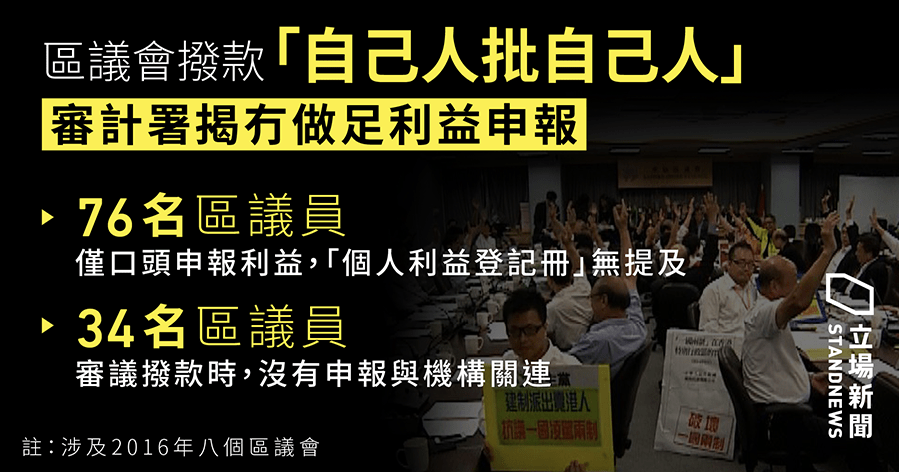
\includegraphics[width=0.7\textwidth]{c26/h-klesson1-043.png}
    \caption{區議會的地區活動經費被指審批不當} 
\end{figure}

區議員的審批能力和利益衝突問題,近年終在「區區一億」事件中被廣泛關注。二零一三年施政報告中提出每區預留一億元推行「社區重點項目計劃」,儘管有個別區議會提出了一些急市民所急的項目,例如推行社區健康服務,但多數項目均受到社區和專業界別的廣泛質疑,被認為是浪費資源和缺乏諮詢。例如觀塘區建議花五千萬興建海濱音樂噴泉,則被批為破壞原有寧靜環境的大白象工程。大埔區議會建議花五千萬提升林村的旅遊設施,除了被當地居民批評無視現有旅客數目已超過交通負荷外,更被揭發有甄選小組成員本身就是興建及營運林村項目公司的董事,最後區議會要在爭議聲中撤回項目。

上述的種種問題揭示的其實是民主失效:負責審批的區議員雖然背負民意代表之名,但他們其實沒有能力做好這代表工作,因為民意在授權時並沒有在意到他們原來有這些職能。樂觀一點去看,只要選民在投票時重新思考區議會的功能和區議員的責任,則上述的問題均可被打破。回看各屆區議會選舉的結果,投票率一般都比立法會選舉為低。再細看選票下跌的幅度,建制陣營的跌幅不大,投票率下跌的主因相信是非建制陣營的支持者沒有出來投票。以沙田瀝源選區為例,非建制陣營在2016年立法會選舉中合共拿了 2,295票,遠多於建制陣營的 1,624 票。但在2015年的區議會選舉中,非建制陣營候選人得 1,406 票,建制陣營候選人得 1,799 票。也就是說,建制陣營可以在區議會選舉中勝出,並不是他們的候選人特色吸引,而是支持非建制陣營的選民不關心區議會選舉。同樣的情況在全港發生,即使建制陣營的候選人的議會表現參差,仍能在區議會勝出。如果沒有投票的那些選民意識到區議會的真正影響,願意出來投票,則區議會選舉可變得有競爭,區議員的質素便才提高。

區議會的案例說明了香港的一個重要問題:香港社會不是太政治化,而是未夠政治化。輿論有時會把民生和政治放在對立面,儘管現實上民生就是政治。即使在區議會的層面,所謂社區其實就是一張由街坊福利會、宗親會、地區團體、屋邨互助委員會和大廈法團,以至政府前線部門如食物環境衛生署和公共事業(例如煤氣公司)等等所組成的關係網。他們之間的互動,各種規則的訂立和背後牽涉到的利益分配,全部都是政治。從社區的整體規劃和建設,到公共空間的管理和利用,到物業維修管理和相關聯的圍標問題,無論居民自己有沒有意識到,政治早就是生活的一部分。與其視而不見,不如好好把握。



伸延閱讀:

費臣(2007):〈區選無間道〉,《明報》2007年11月7日。

金佩瑋(2013):〈社區建設八大支柱〉,張少強、梁啟智、陳嘉銘編《香港.論述.傳媒》,香港:牛津大學出版社。

網上資源:

\href{https://thestandnews.com/society/不能避雨亭-之父-民建聯區議員丁江浩-設計圖美觀-製成品有出入/ }{立場報道(2015)「不能避雨亭」 之父 民建聯區議員丁江浩:設計圖美觀 製成品有出入,2015年5月7日}

\href{https://www.thestandnews.com/politics/審計報告-34區議員討論撥款時-無申報利益/}{立場報道(2017)34區議員傾撥款無申報利益 六成申報個案主席無裁決 有利益者會照開,2017年4月26日}